\documentclass[../../submission.tex]{subfiles}
\begin{document}
\section{Result}
This section presents the findings of our user study, evaluating the performance of an 
AI-driven natural language interface (NLI) against a conventional search system in 
an e-commerce context. The results address user satisfaction, the role of filters, 
technical feasibility, and possible correction mechanisms for query optimization, providing insights 
into the effectiveness of dynamic SQL query generation compared to static templates.

\subsection{User Satisfaction and Search Behavior(RSQ1)}
As shown in Figure \ref{fig:result_AI}, all participants expressed higher satisfaction with the 
AI-driven system’s results, with responses on a 5-point Likert scale ranging from 
'satisfied' to 'very satisfied.' Specifically, 69\% (9 out of 13 participants) 
rated their satisfaction as very high (1/5), and 31\% (4 out of 13) as high (2/5). 
The mean satisfaction score was 1.69 (SD = 0.48, calculated with bessel correction), indicating low variability in responses. Due to the small sample size (n=13), statistical significance tests were not conducted.
 Users highlighted the system’s ability 
to accurately interpret their search intent as a key factor in their positive experience. 
Notably, the AI’s capability to handle typographical errors and synonyms was well-received. 
For example, it recognized 'Wiener Dog' as 'Dachshund,' as shown in Figure \ref{fig:wiener_dog}. 
This feature was absent in the conventional system.

\begin{figure}[h]
    \centering
    \begin{minipage}{0.45\textwidth}
        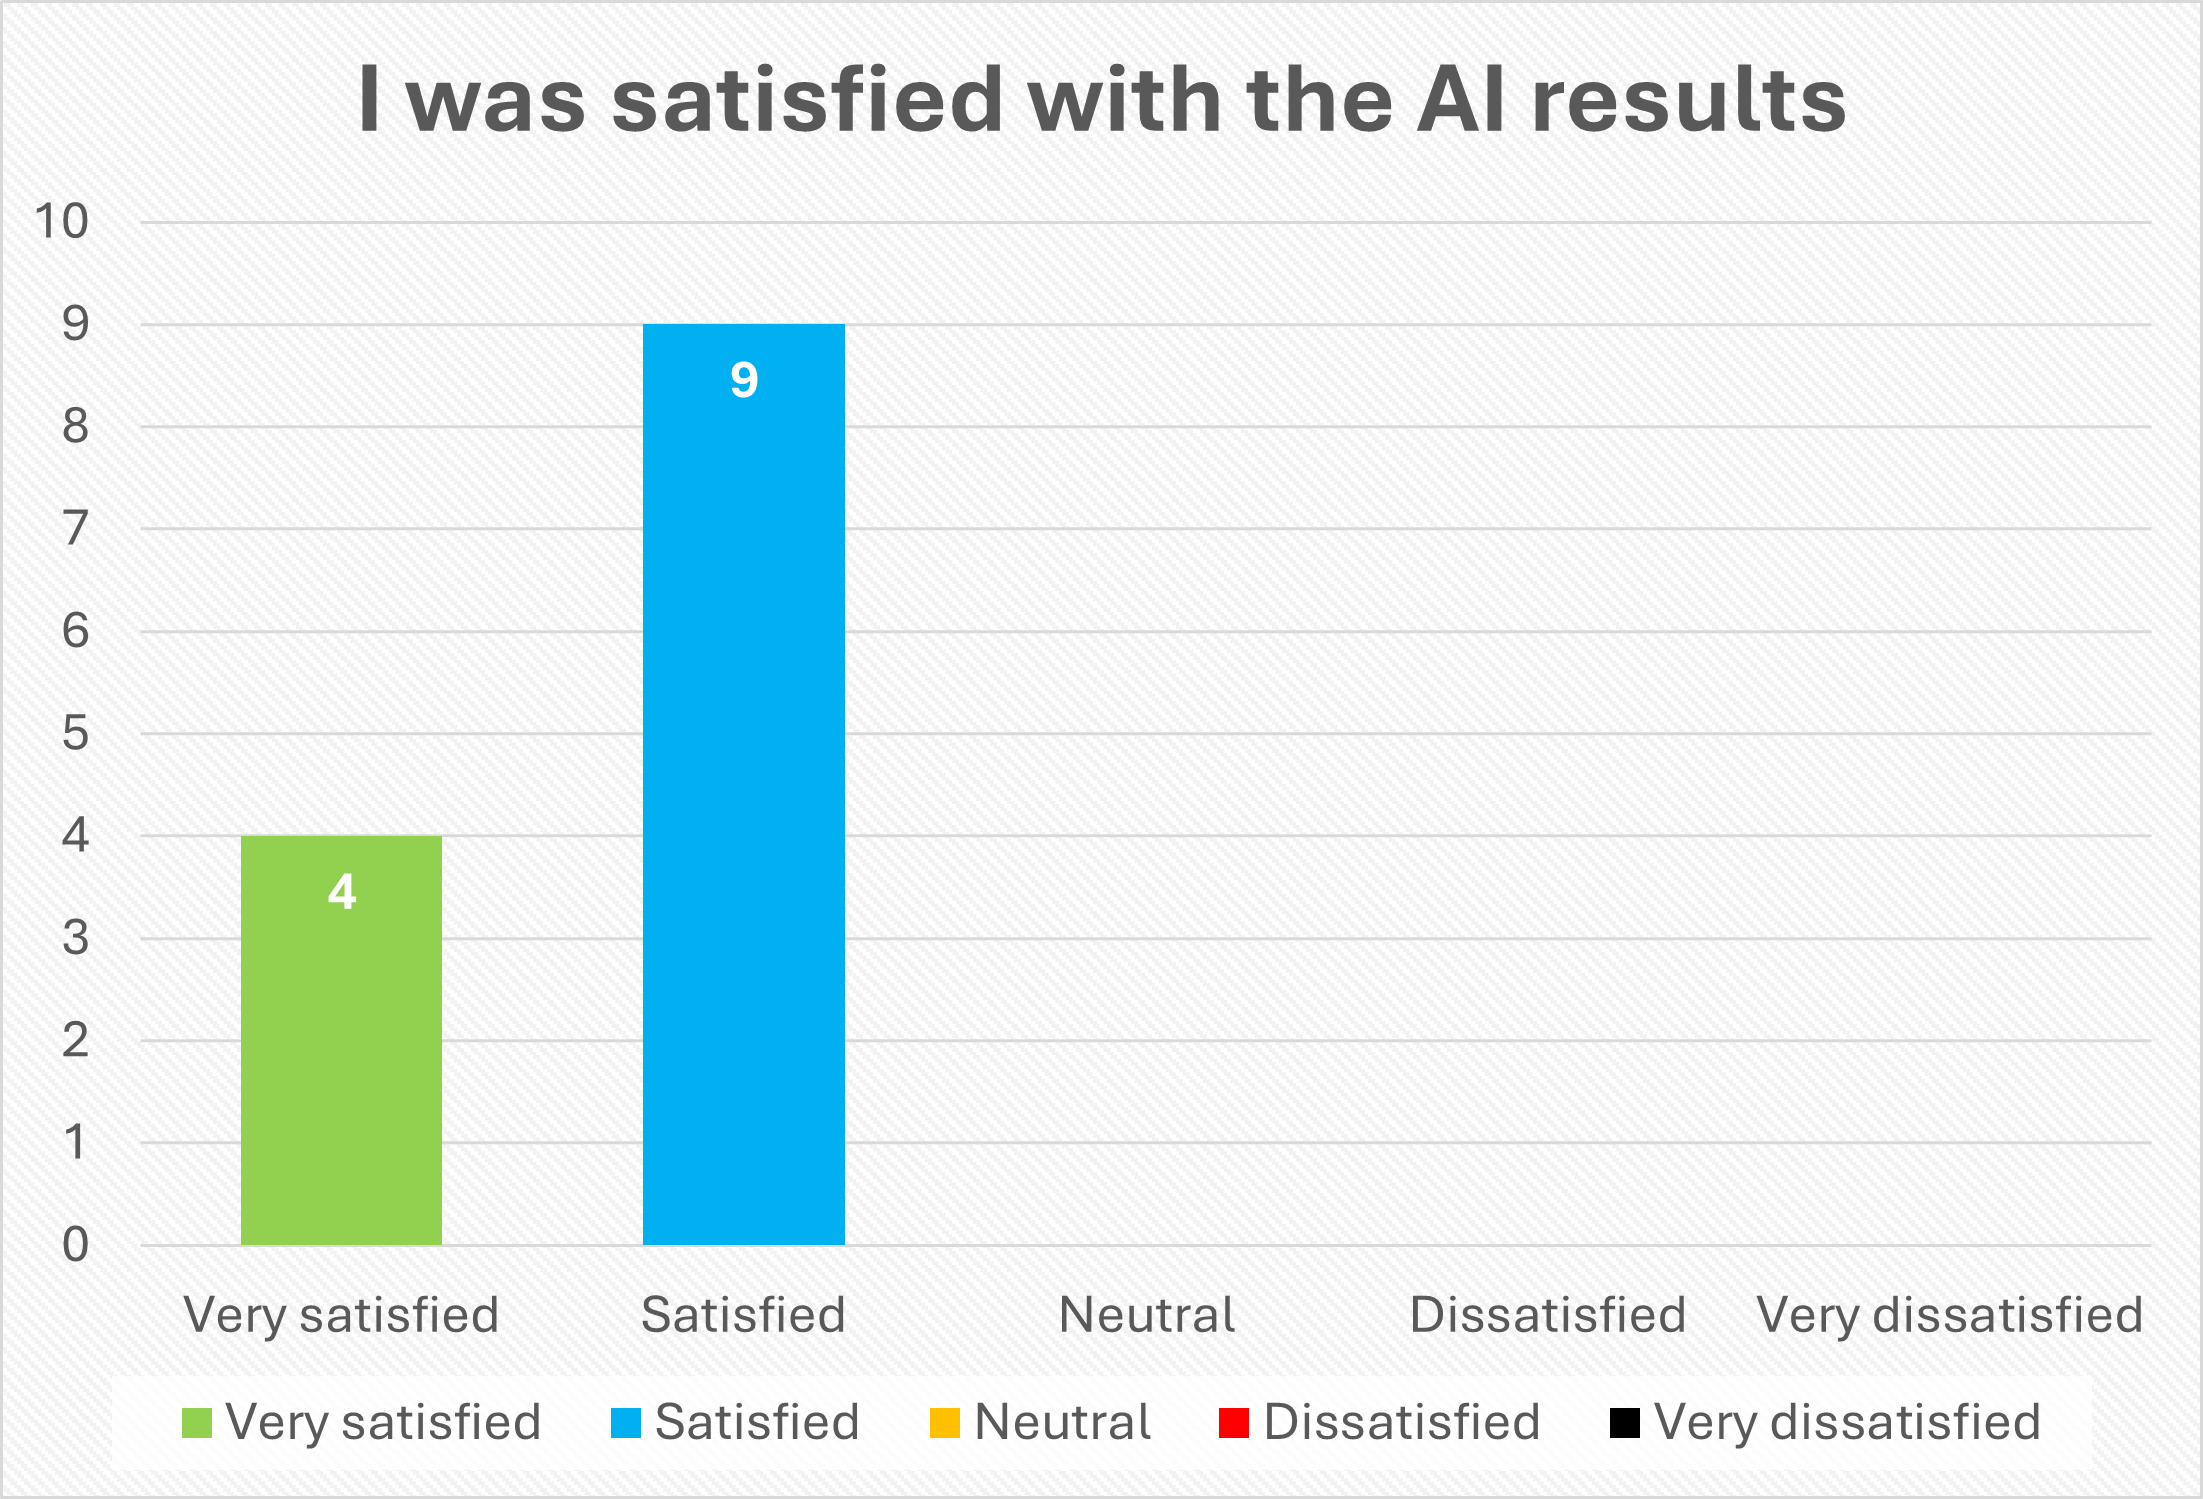
\includegraphics[width=\textwidth]{images/result_ki}
        \caption{The users' rating regarding the satisfaction of the results displayed by the AI. As can be seen in the picture, the participants were very satisfied with the results of the AI.}
        \label{fig:result_AI}
    \end{minipage}
    \hfill
    \begin{minipage}{0.45\textwidth}
        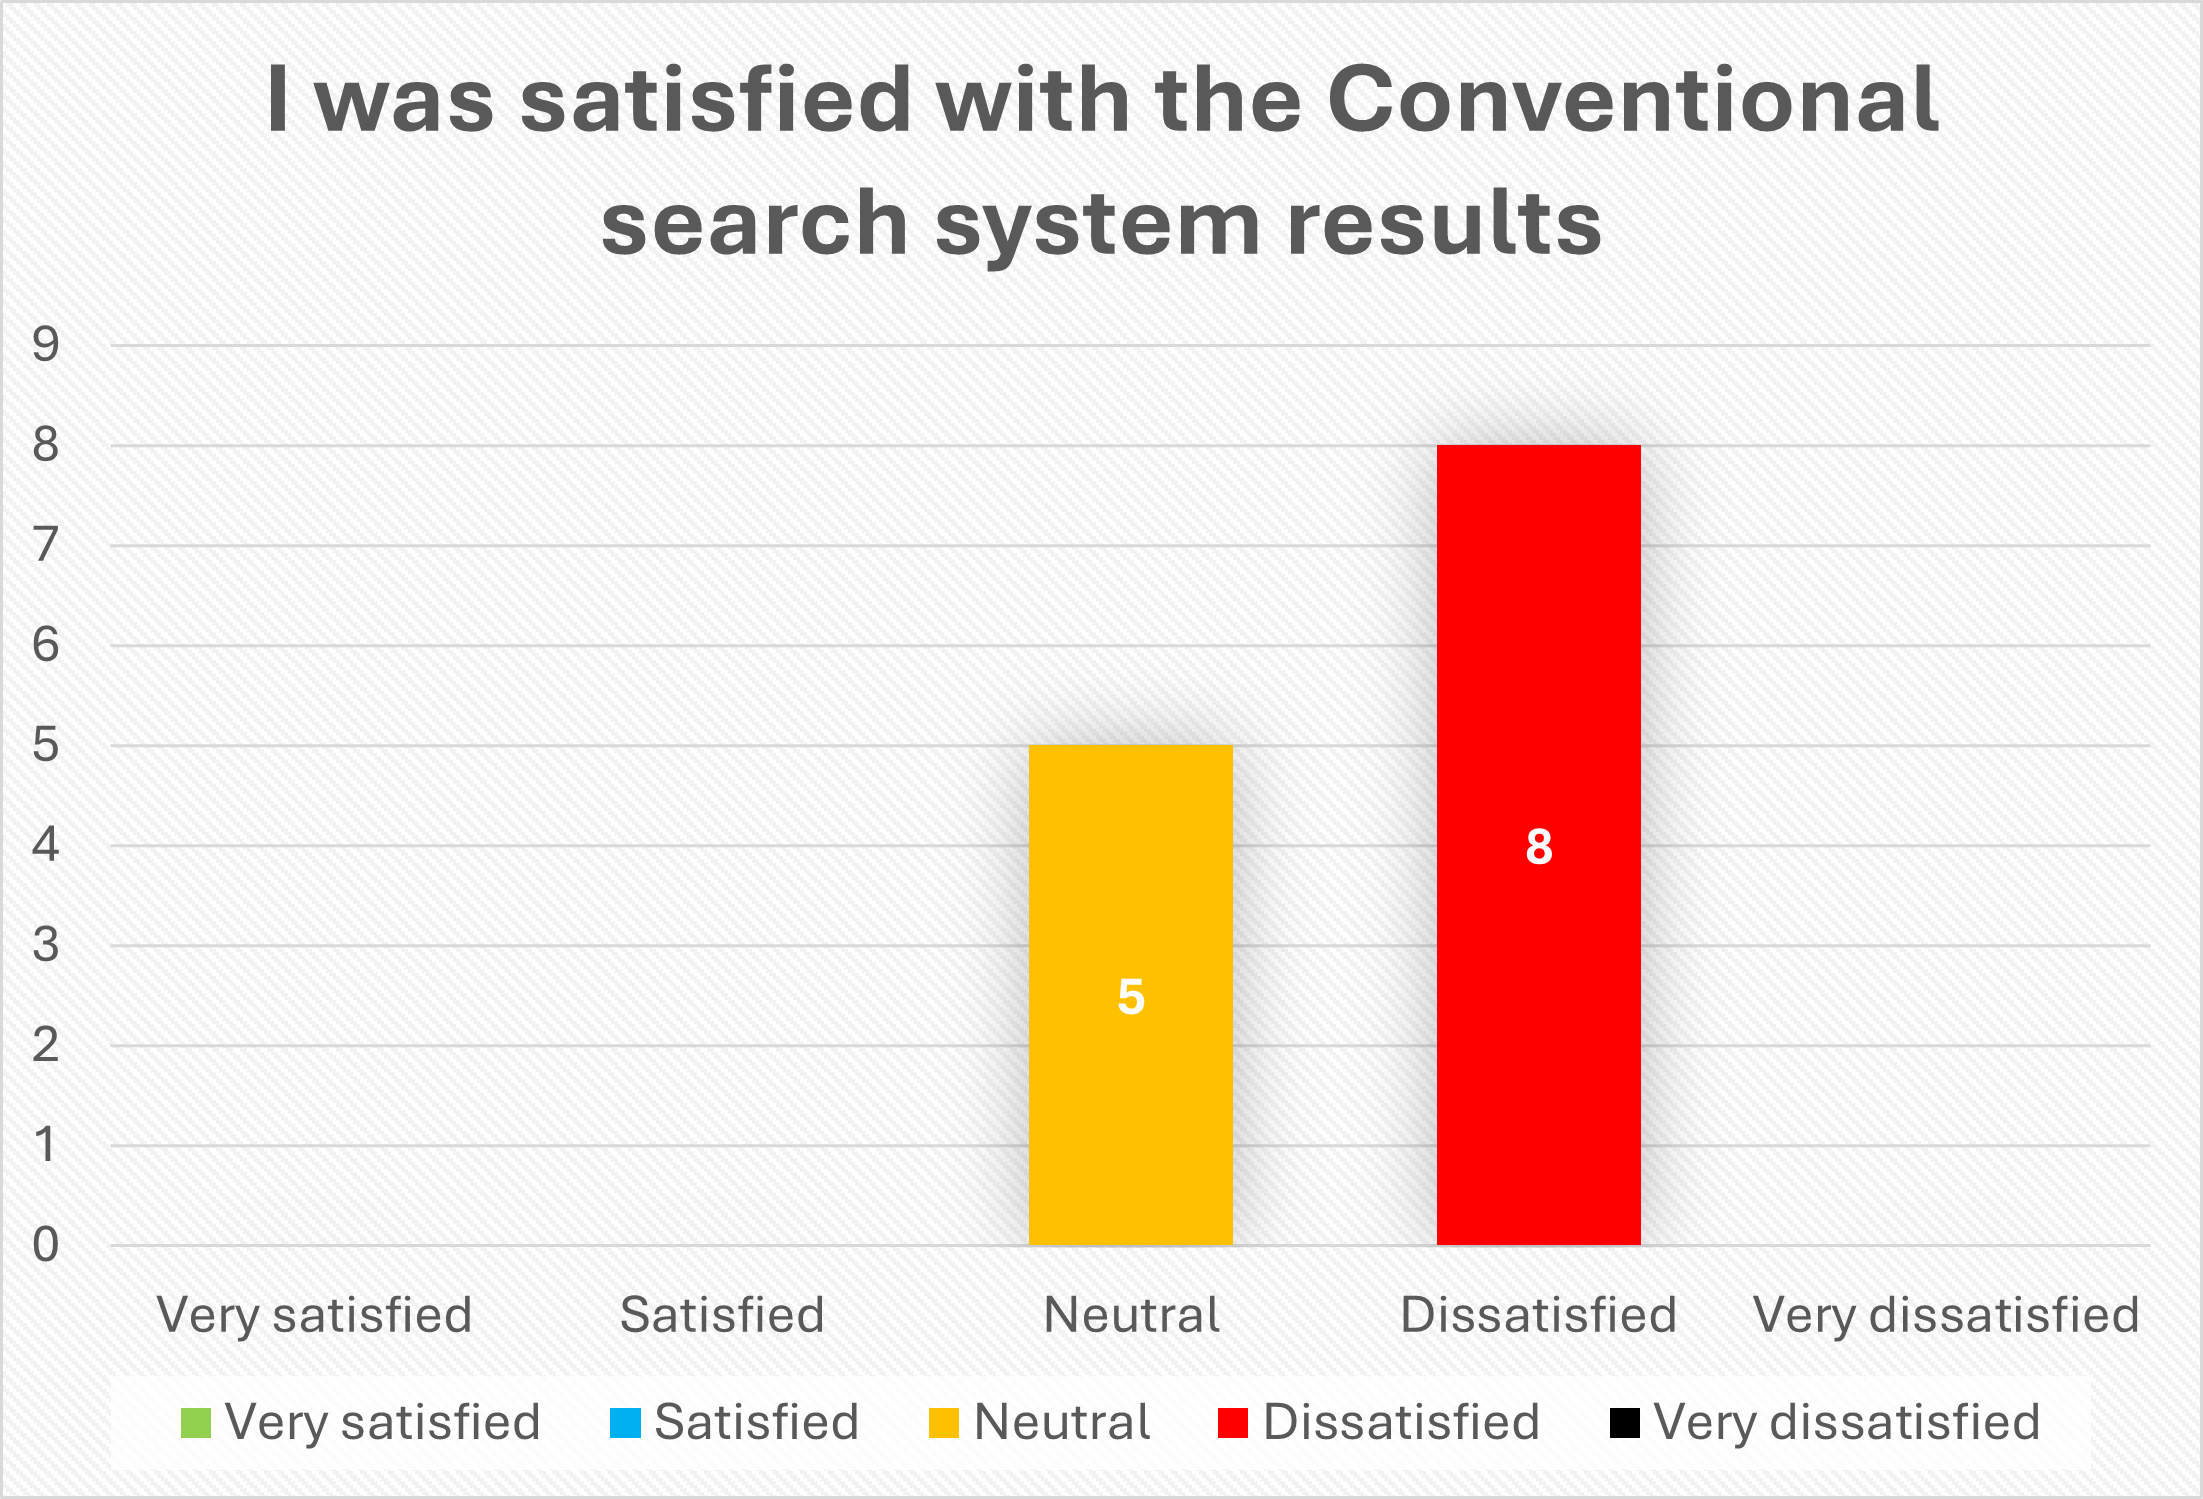
\includegraphics[width=\textwidth]{images/result_konv}
        \caption{The evaluation of the users regarding the satisfaction with the result displayed by the conventional system. The picture shows that they were not satisfied with the results displayed by the conventional system.}
        \Description{}
        \label{fig:result_Konv}
    \end{minipage}
\end{figure}
 
In contrast, satisfaction with the conventional 
system was markedly lower, averaging 3.62(SD = 0.51) on the same scale, with only 38\% (5 out of 13) rating it as neutral (3/5), and 62\% 
(7 out of 13) as dissatisfied (4/5), with no participants rating it as very high,high or 
very dissatisfied (see Figure \ref{fig:result_Konv}). Users found its performance lacking, particularly when compared to the AI’s 
intuitive query handling. An interesting observation emerged: as participants grew 
accustomed to the AI’s ability to understand their intent, their reliance on manual 
filters decreased. This shift likely contributed to the conventional system’s perceived 
inferiority, as it depended heavily on filter usage to refine results. This rapid 
adaptation suggests a potential change in search behavior, though further analysis is 
needed to confirm its extent. 


\begin{figure}[h]
    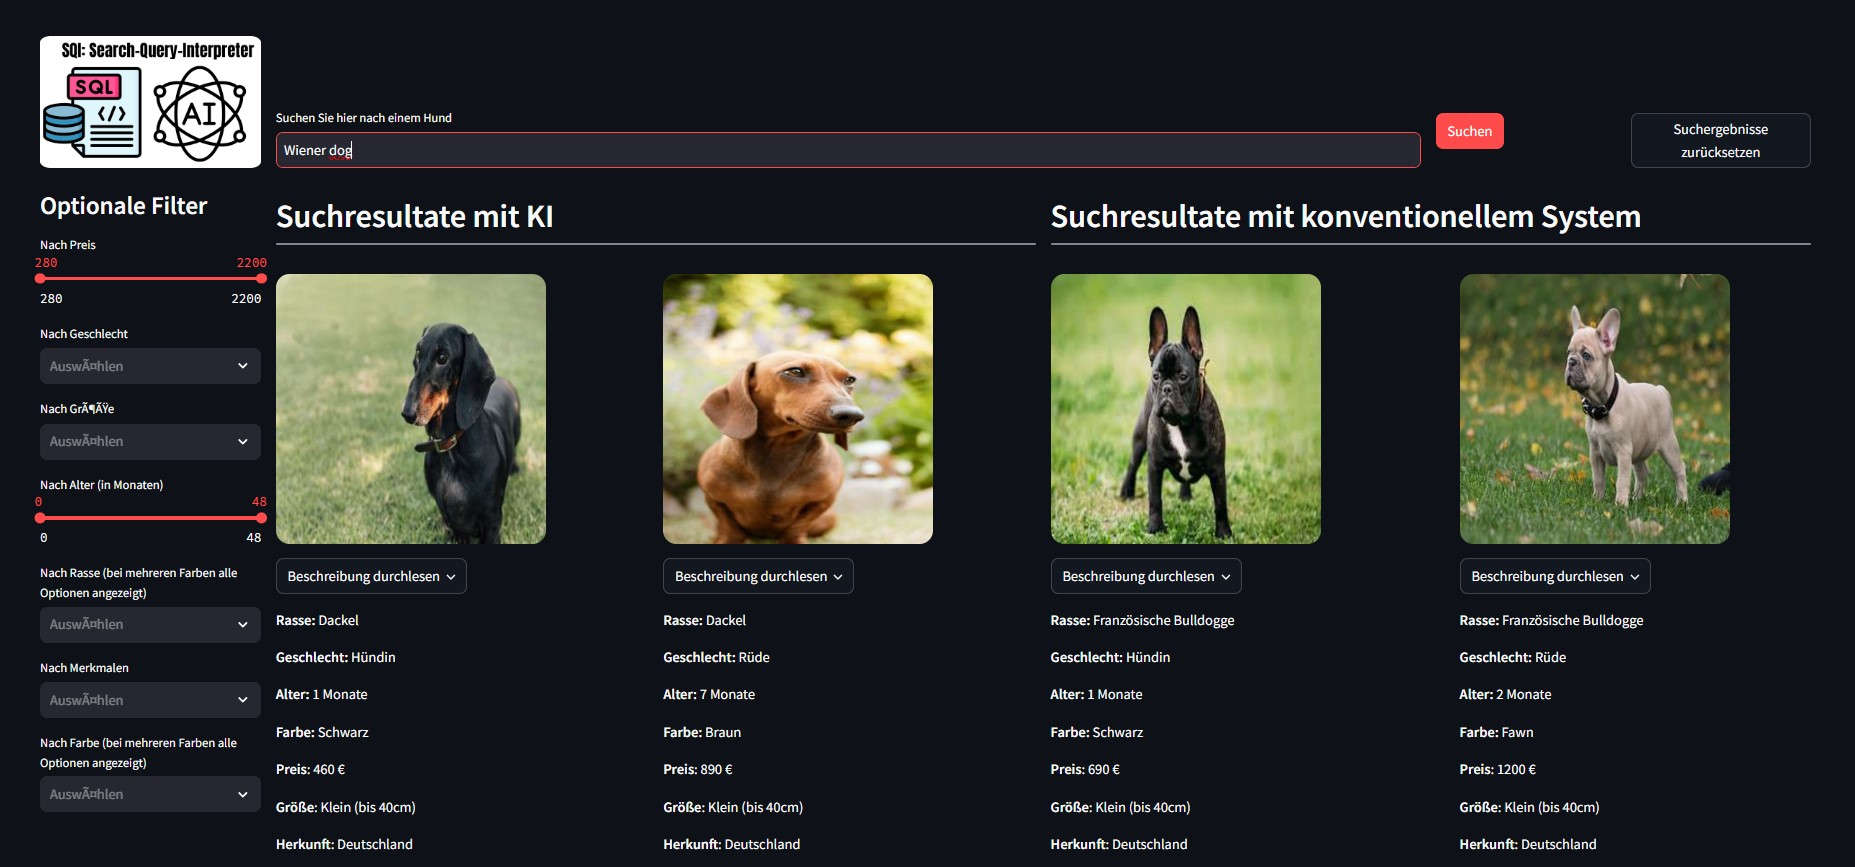
\includegraphics[width=0.7\textwidth]{images/wiener_dog}
    \caption{In this picture we see the website that was developed for the project. The website was divided so that the user can quickly see which results belong to AI and which to the conventional system. To demonstrate the performance of the AI, Wiener dog was entered in the input field. As you can see, the AI can handle this, but the conventional system cannot.}
    \Description{}
    \label{fig:wiener_dog}
 \end{figure} 

 It’s worth noting that the results for the conventional 
system should be considered in light of the relatively simple static template we used. 
This basic design may have contributed to its poorer performance, and a more sophisticated 
static template could potentially have yielded better outcomes.

 \subsection{The Role of Filters in Enhancing User Experience}
 Despite the AI’s potential to replace traditional filtering mechanisms, our study 
 revealed that filters retained significant relevance for users. 
 Figure \ref{fig:without_filter} shows participants’ preferences regarding filter usage in the AI-driven 
 system, based on a 5-point Likert scale (1 = ‚strongly agree‘, 5 = ‚strongly disagree‘) 
 from the post-study questionnaire. Of the 13 participants, 9 (69.2\%) agreed or 
 strongly agreed they could manage without filters (scores 1–2), 3 (23.1\%) 
 disagreed, preferring to retain them (scores 4), and 1 (7.7\%) selected ‚neutral‘ 
 (score 3).
 Of the participants who preferred filters, three stated in open-ended comments 
 that they appreciated the visual clarity, such as when sorting by price or selecting 
 ranges (e.g., ‘price between 50-100€’), compared to text-based inputs. 
 For instance, participants noted that setting a price range via a slider was 
 faster and more intuitive than specifying it textually.
 These findings, however, are based on a small, homogeneous sample of 13 participants, 
primarily computer science students, which may limit generalizability.



 \begin{figure}[h]
    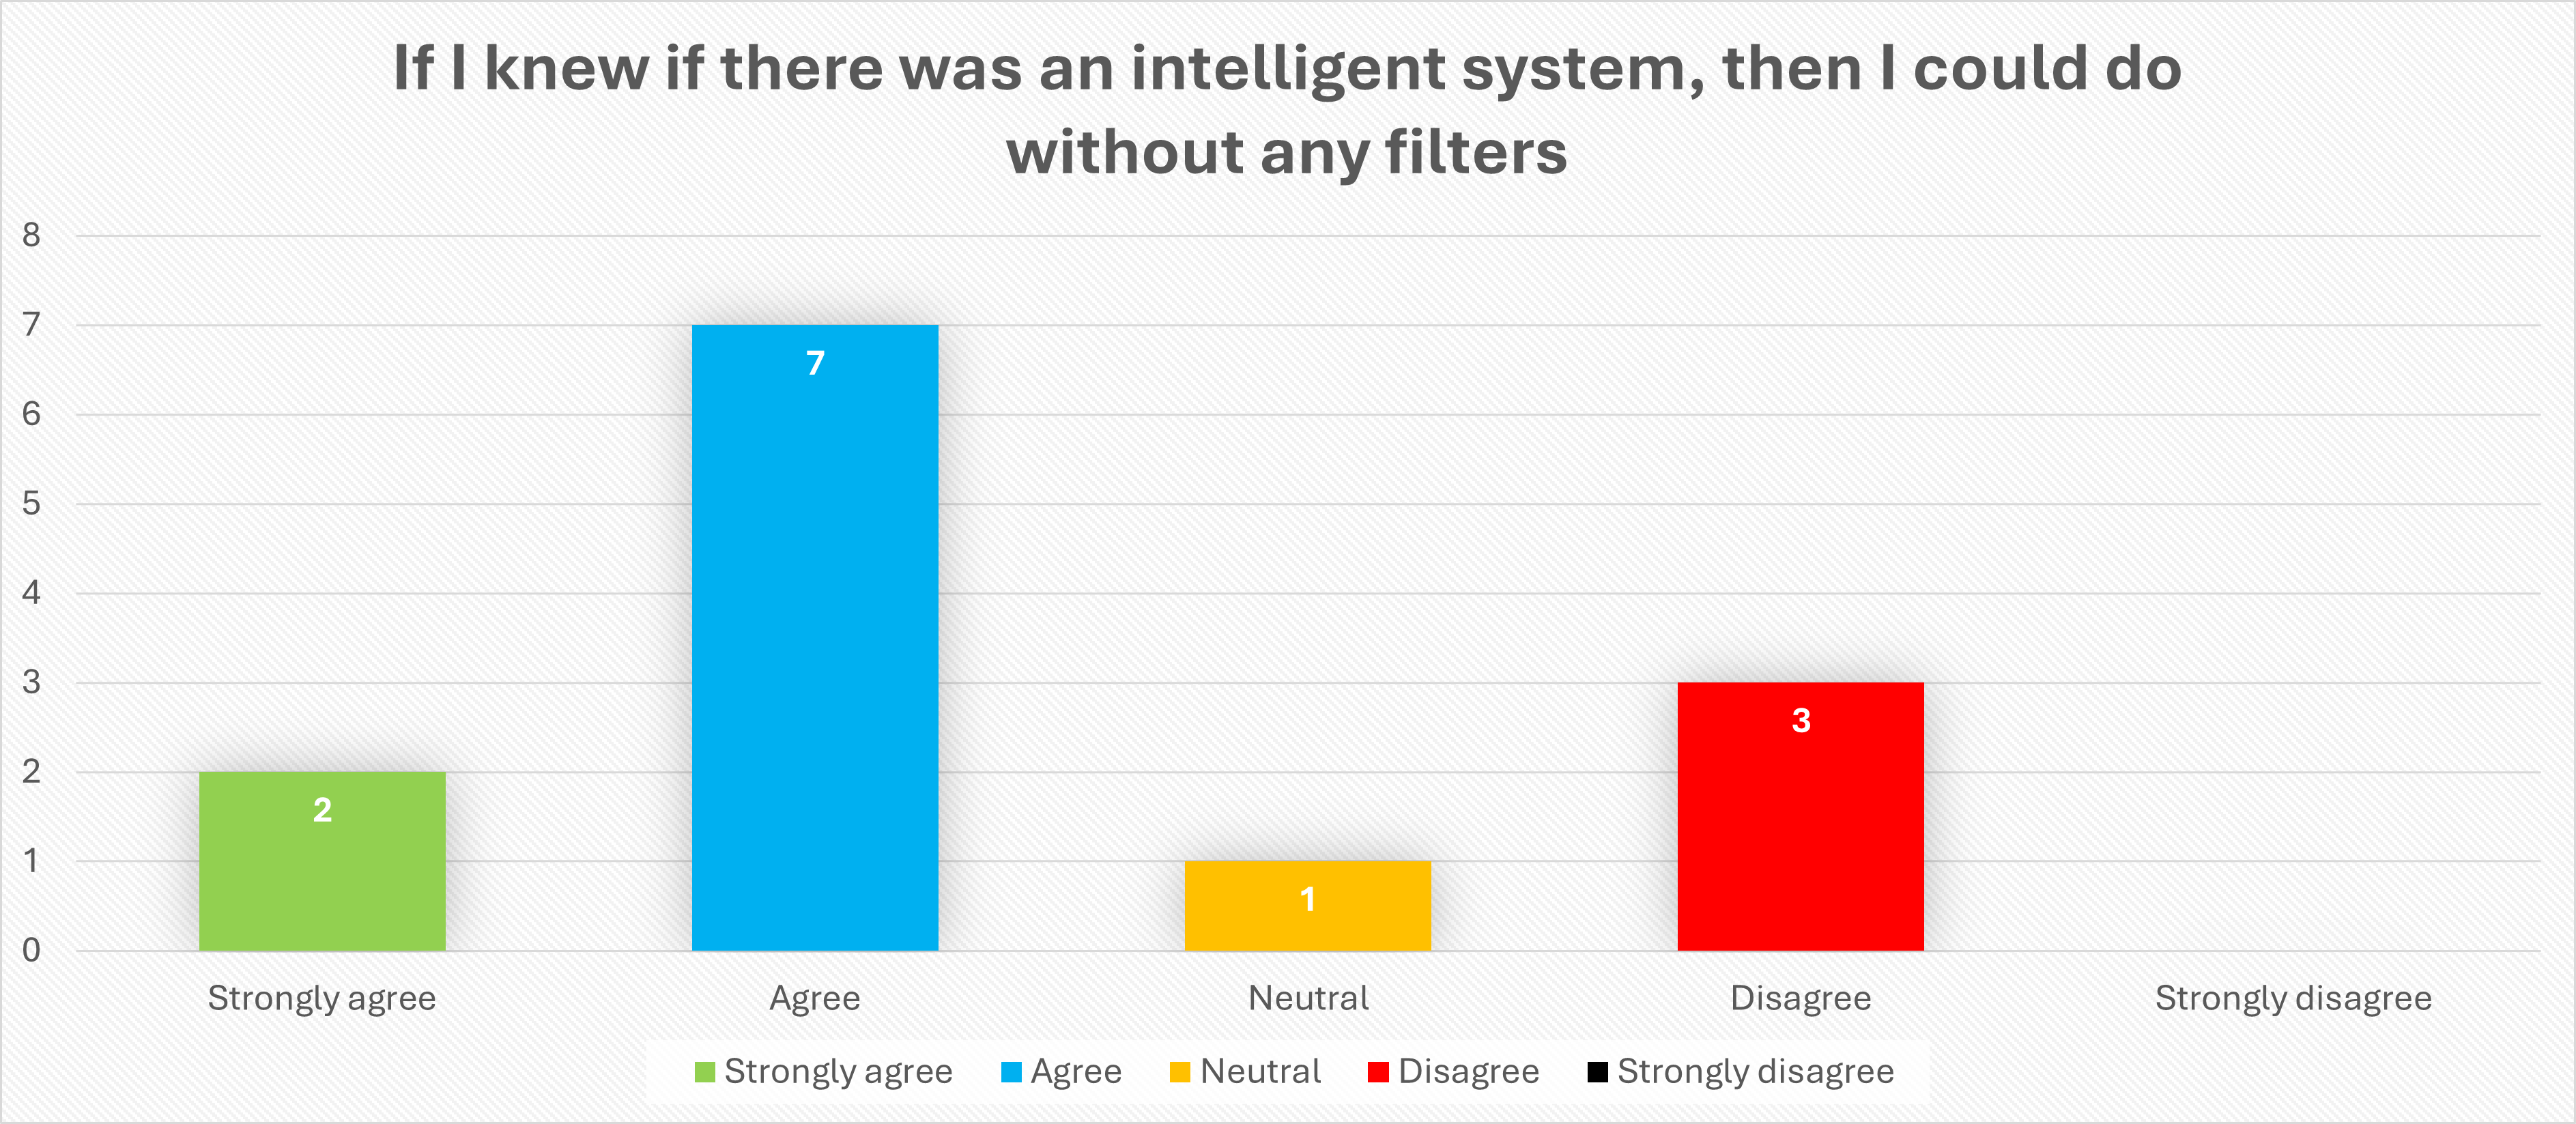
\includegraphics[width=\textwidth]{images/without_filter}
    \caption{After the users have used the system, they should state whether they would manage without the filter.The results show that the majority of users can manage without a filter without any problems. Three times “disagree” was indicated, while no “strongly disagree” was recorded.}
    \Description{}
    \label{fig:without_filter}
 \end{figure}

 \subsection{Technical Feasibility and Security Considerations (RSQ2)}
 Building on user experience insights, this subsection examines the technical implications 
 of the AI-driven system. During the study, some participants tested the system’s boundaries, 
 revealing critical security concerns. For example, one user entered a command to 'delete 
 all tables,' which the AI translated into an executable SQL query—an unintended capability 
 that exposed a vulnerability. Ideally, the system should restrict operations to read-only 
 searches, preventing modifications to the database or its schema. While our simple dog 
 webshop schema excluded sensitive data like user information, real-world applications 
 would demand robust safeguards. We propose implementing a security mechanism using 
 Prepared Statements, which bind user inputs to predefined query structures, preventing 
 malicious commands from being executed. Alternatively, a whitelist of permitted SQL 
 operations (e.g., SELECT only) could ensure that generated queries remain safe, enhancing 
 both functionality and security. 

 To address this, we propose implementing a log file-based blacklist to enhance security. 
 This approach would involve maintaining a record of prohibited words, such as specific 
 table names or keywords like "delete" or "drop," that the AI is not permitted to include 
 in its output. Before executing any generated SQL query, the AI could cross-check its 
 commands against this blacklist. If a match is detected, the query would be blocked, 
 preventing potentially harmful operations. This mechanism would safeguard both the 
 integrity of the data and the security of the database, offering a practical layer 
 of protection while preserving the system’s functionality for legitimate search tasks.
 
 \subsection{Optimizing Query Correction Strategies (RSQ3)}
 To address usability challenges and enhance trust, we investigated user preferences 
 for refining inaccurate search results. Participants suggested several strategies, 
 detailed below, to improve the system’s transparency and responsiveness.

 \begin{figure}[h]
     \centering
     \begin{minipage}{0.40\textwidth}
        \subsubsection{Dynamic Filter Adjustment}
        A participant has proposed an adjustment of the filters, based on the input provided. As illustrated in Figure \ref{fig:filter}, 
        the idea is to highlight implicitely used filters visually, i.e. dynamically adjusting filters on the interface. 
        Therefore, the user is able to ascertain 
        which filters the AI utilizes and, consequently, identify the potential origin of an error. Therefore, the user 
        has the option of either utilize the filter to resolve the issue or adjusting the initial search query.       
     \end{minipage}
     \hfill
     \begin{minipage}{0.43\textwidth}
        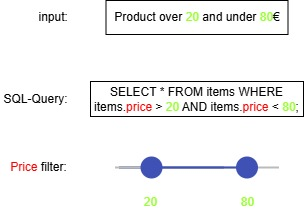
\includegraphics[width=\textwidth]{images/filter}
        \caption{Here the user can see how the filter is adapted to the user's input. The filter adapts to user input, revealing AI misinterpretations (implicitely).}
        \Description{}
        \label{fig:filter} 
    \end{minipage}
 \end{figure}



 \begin{figure}[h]
    \centering
    \begin{minipage}{0.35\textwidth}
        \subsubsection{User Notification for No Results}
        A further potential avenue for enhancing the efficancy of the user's 
        outcomes is the implementation of an artificial intelligence system that can 
        evaluate the combinability of diverse features during the user's input phase. 
        In such a case, it is essential that the user be alerted to this possibility. 
        The current state of the AI, reflecting the original user input, is shown in Figure \ref{fig:no_result}. The subsequent version has been enhanced to alert the user to the 
        absence of search results for a given combination of features. In this instance, the 
        "under 2 months" feature is distinctly emphasized, as it does not result in any search results. 
        Therefore, the user has the capacity to modify the preliminary search query and discern the 
        elements that are not compatible.  
    \end{minipage}
    \hfill
    \begin{minipage}{0.55\textwidth}
        
        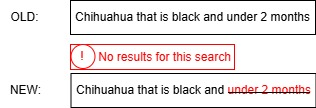
\includegraphics[width=\textwidth]{images/keine_ergebnisse}
        \caption{Here the user is informed by the AI if the features are not combinable. It is made clear that ‘under 2 months’ cannot be combined with the other features, as this feature is crossed out.}
        \Description{}
        \label{fig:no_result}
    \end{minipage}
\end{figure}

\subsubsection{Display of Similar Results}   

A further point to be considered is the potential for the AI to present analogous
 products in the event that the search yields few results. A relevant example  
 would be a search for dogs that are of medium size. In the event that the available 
 results are limited, the artificial intelligence could be programmed to display dogs of 
 smaller stature.

\begin{figure}[h]
    \centering
    \begin{minipage}{0.35\textwidth}
        \subsubsection{Real-time AI-driven Suggestions}
        Another idea for improving the system is to offer the user search suggestions as they type. 
        This not only enables the AI to deliver more relevant results, but also to better understand what the user is looking for.
        An example of this is shown in Figure \ref{fig:suggestions}. The user enters 'Puppy that is black and...' and the AI suggests narrowing the 
        search - for example to 'Puppy that is black and under three months'.
    \end{minipage}
    \hfill
    \begin{minipage}{0.55\textwidth}
        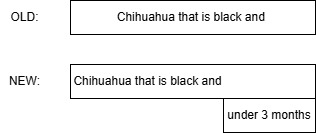
\includegraphics[width=\textwidth]{images/vorschlag}
        \caption{The AI provides real-time suggestions for narrowing searches, such as additional features for 'Chihuahuas'.}
        \Description{}
        \label{fig:suggestions}
    \end{minipage}
\end{figure}
 

 
 \subsubsection{Query Confidence Indicator}   
 
 Another suggestion from users is that the AI should more clearly indicate its uncertainty 
 when interpreting a query, for example, by providing an uncertainty score/confidence ranging from 
 0 to 1. This score would reflect how confident the AI is in its understanding of the 
 request. This would allow users to better assess whether the provided results might 
 be inaccurate or incorrect, enabling them to make adjustments if needed.

 An example from the current AI system illustrates this. When a user searches for 
 a “cheap dog,” the AI often simply returns the least expensive dog available. 
 However, this may not align with what the user intended; perhaps they were looking 
 for a cost-effective yet suitable dog for specific needs. An uncertainty score could 
 indicate how reliable the results are, signaling to the user that the interpretation 
 of their query might not be entirely accurate. This would give the user the opportunity 
 to refine their request for more appropriate responses.

\end{document}